\section{互信息作为依赖量}
\label{sec:dep-mutual-information}

第~\ref{chap:information-measures}章已经给出一个直接比较式~\eqref{eq:dep-independence}两边的量。设$X,Y$分别取值于可测空间$\mathcal{X},\mathcal{Y}$，互信息定义为联合分布相对边缘乘积的KL散度，
\begin{equation}
  I(X;Y)=D_{\mathrm{KL}}\bigl(P_{(X,Y)}\,\Vert\,P_X\otimes P_Y\bigr)\in[0,\infty].
  \label{eq:dep-mi}
\end{equation}
按第~\ref{chap:distribution-comparison}章的约定，若$P_{(X,Y)}$不绝对连续于$P_X\otimes P_Y$，KL散度取$+\infty$。那里也证明了KL散度非负、且为零当且仅当两个分布相同，所以
\[
  I(X;Y)=0\iff P_{(X,Y)}=P_X\otimes P_Y\iff X\text{与}Y\text{独立}.
\]
零值判据不需要任何矩条件，也不需要$\mathcal{X},\mathcal{Y}$是欧氏空间。在离散情形，式~\eqref{eq:dep-mi}写成概率表上的求和
\[
  I(X;Y)=\sum_{x,y}p_{X,Y}(x,y)\ln\frac{p_{X,Y}(x,y)}{p_X(x)\,p_Y(y)},
\]
零概率的格子按$0\ln0=0$不计入。

用三点抛物线算一遍。联合表只有三个正格子，每个概率为$1/3$。格子$(\pm1,1)$处边缘乘积为$\frac13\cdot\frac23=\frac29$，格子$(0,0)$处为$\frac13\cdot\frac13=\frac19$。代入求和式，
\[
  I(X;Y)=2\cdot\frac13\ln\frac{1/3}{2/9}+\frac13\ln\frac{1/3}{1/9}=\frac23\ln\frac32+\frac13\ln3 .
\]
整理成一个数，
\[
  I(X;Y)=\ln3-\tfrac23\ln2\approx0.637\ \text{nat}.
\]
它恰好等于$Y$的熵$H(Y)=\frac13\ln3+\frac23\ln\frac32$：$Y$由$X$确定，观测$X$后$Y$的不确定性全部消失，减少量就是$Y$原有的不确定性。

互信息的熵差表示、链式法则和计算下界都在第~\ref{chap:information-measures}章，这里不再重复。下面关心的是：把互信息当作依赖的强弱刻度时，它对坐标变换怎样反应，数值能大到什么程度。

\subsection{变换不变性}
\label{sec:dep-mi-invariance}

把$Y$的两个取值$0,1$改名为“短”“长”，或者把温度从摄氏度换成华氏度，两个变量之间的依赖不应当改变。互信息正好如此。所用的工具是第~\ref{chap:information-measures}章的数据处理不等式：若$Z$只通过$Y$依赖$X$，即给定$Y$时$X$与$Z$条件独立，则$I(X;Z)\leq I(X;Y)$。$Z=g(Y)$由$Y$确定，这个条件自动成立。

\begin{theorem}[互信息的变换性质]
\label{thm:dep-mi-invariance}
设$f:\mathcal{X}\to\mathcal{X}'$与$g:\mathcal{Y}\to\mathcal{Y}'$可测。
\begin{enumerate}
  \item 局部处理不增加互信息：
  \begin{equation}
    I\bigl(f(X);g(Y)\bigr)\leq I(X;Y).
    \label{eq:dep-mi-processing}
  \end{equation}
  \item 若$f$与$g$都是双向可测的一一映射（逆映射也可测），则
  \begin{equation}
    I\bigl(f(X);g(Y)\bigr)=I(X;Y).
    \label{eq:dep-mi-invariance}
  \end{equation}
\end{enumerate}
\end{theorem}

\begin{proof}
先处理$Y$一侧。$g(Y)$是$Y$的函数，由数据处理不等式，$I(X;g(Y))\leq I(X;Y)$。互信息关于两个变量对称，对$X$一侧同样有$I(f(X);g(Y))\leq I(X;g(Y))$。两步相连，
\[
  I\bigl(f(X);g(Y)\bigr)\leq I\bigl(X;g(Y)\bigr)\leq I(X;Y),
\]
这就是式~\eqref{eq:dep-mi-processing}。

若$f,g$双向可测且一一，则$X=f^{-1}(f(X))$、$Y=g^{-1}(g(Y))$，对变量$f(X),g(Y)$与可测映射$f^{-1},g^{-1}$再用一次式~\eqref{eq:dep-mi-processing}，
\[
  I(X;Y)=I\bigl(f^{-1}(f(X));\,g^{-1}(g(Y))\bigr)\leq I\bigl(f(X);g(Y)\bigr).
\]
与第一部分相反方向的不等式合起来，得到式~\eqref{eq:dep-mi-invariance}。
\end{proof}

\paragraph{改名与改坐标}
在三点抛物线中，把$X$的取值$-1,0,1$换成$-1,0,5$，或把$Y$的取值$0,1$换成$0,100$，概率表的格局完全不变，互信息仍是$\ln3-\frac23\ln2$。互信息只看“哪些取值一起出现、各占多少概率”，不看取值之间相距多远。这既是长处也是局限：它不受单位和刻度影响，但也不反映“$Y$随$X$变化了多少”。

连续变量的例子是标准二元高斯$(X,Y)$，相关系数$\rho=0.5$，协方差矩阵$\bm{\Sigma}$的对角元为$1$、非对角元为$\rho$。$d$维高斯向量的微分熵是$\frac12\ln\bigl((2\pi\mathrm{e})^{d}\det\bm{\Sigma}\bigr)$，用第~\ref{chap:information-measures}章的熵差表示$I(X;Y)=h(X)+h(Y)-h(X,Y)$，常数项相消，只剩
\begin{equation}
  I(X;Y)=-\tfrac12\ln\det\bm{\Sigma}=-\tfrac12\ln(1-\rho^{2}).
  \label{eq:dep-gauss-mi}
\end{equation}
$\rho=0.5$时它等于$-\frac12\ln0.75\approx0.144$ nat。
对两个坐标分别作严格增变换$x\mapsto\mathrm{e}^{x}$，得到对数正态向量$(\mathrm{e}^{X},\mathrm{e}^{Y})$。它的相关系数由高斯的矩母函数算出。$X+Y$的方差为$2+2\rho$，所以
\[
  \mathbb{E}[\mathrm{e}^{X}]=\mathrm{e}^{1/2},\qquad \mathbb{E}[\mathrm{e}^{2X}]=\mathrm{e}^{2},\qquad \mathbb{E}[\mathrm{e}^{X+Y}]=\mathrm{e}^{1+\rho}.
\]
于是
\[
  \operatorname{Corr}\bigl(\mathrm{e}^{X},\mathrm{e}^{Y}\bigr)=\frac{\mathrm{e}^{1+\rho}-\mathrm{e}}{\mathrm{e}^{2}-\mathrm{e}}=\frac{\mathrm{e}^{\rho}-1}{\mathrm{e}-1}\approx0.378 .
\]
相关系数从$0.5$降到$0.378$，互信息由定理~\ref{thm:dep-mi-invariance}保持$0.144$不变。

\paragraph{只依赖Copula}
再换一种坐标：用分布函数把两个分量都送到$(0,1)$上，$(U,V)=(\Phi(X),\Phi(Y))$。这正是第~\ref{chap:distribution-families}章的概率积分变换，$(U,V)$的分布是$\rho=0.5$的高斯Copula。$\Phi$连续且严格增，是双向可测的一一映射，所以$I(U;V)=I(X;Y)$。一般地，若$X,Y$为实值、分布函数$F_X,F_Y$连续，则$U=F_X(X)$与$X$只差一个零概率事件上的取值（$X=Q_X(U)$几乎必然成立，$Q_X$为分位数函数），同样两次运用数据处理得到
\[
  I(X;Y)=I\bigl(F_X(X);F_Y(Y)\bigr).
\]
连续边缘下，互信息只依赖Copula，与边缘分布无关；若Copula有密度$c$，它就是$\int_{[0,1]^{2}}c\ln c$。图~\ref{fig:dep-mi-coordinates}把同一组高斯样本画在三种坐标下：点云形状差别很大，相关系数分别为$0.5$、$0.378$、$0.483$，互信息都是$0.144$。

\begin{BookInlineFigure}
  \centering
  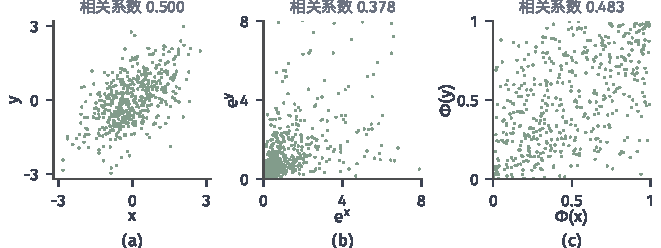
\includegraphics[width=112mm]{figures/07-probability/04-distribution-analysis/matplotlib/dep-mi-coordinates/figure.pdf}
  \caption{同一组标准二元高斯样本（$\rho=0.5$，$500$个，种子$719$）在三种坐标下。(a)原坐标；(b)$(\mathrm{e}^{x},\mathrm{e}^{y})$，有$15$个点超出画框；(c)$(\Phi(x),\Phi(y))$，即高斯Copula。图上方是各自的相关系数$\rho$、$(\mathrm{e}^{\rho}-1)/(\mathrm{e}-1)$与$(6/\pi)\arcsin(\rho/2)$；三者的互信息都是$-\frac12\ln0.75\approx0.144$。}
  \label{fig:dep-mi-coordinates}
\end{BookInlineFigure}

\paragraph{不可逆的处理}
若$f$不是一一的，式~\eqref{eq:dep-mi-processing}一般是严格不等式。在三点抛物线中只保留$X$是否为正，令$B=\mathbf{1}_{\{X>0\}}$。$B=1$时$X=1$，$Y=1$确定；$B=0$（概率$2/3$）时$X$等可能为$-1$或$0$，$Y$等可能为$1$或$0$，剩下$\ln2$的不确定性。于是
\[
  H(Y\mid B)=\tfrac23\ln2,\qquad I(B;Y)=H(Y)-H(Y\mid B)=\ln3-\tfrac43\ln2\approx0.174 .
\]
从$0.637$降到$0.174$：把$-1$和$0$合并以后，原来能区分的情形不再能区分。如果只合并$X$的$-1$与$1$，即改用$\lvert X\rvert$，那么$Y=\lvert X\rvert$仍由它确定，互信息不变。是否损失信息，看被合并的取值对另一个变量是否“有区别”。

\subsection{确定关系与无穷信息}
\label{sec:dep-mi-infinite}

三点抛物线的互信息是有限的$0.637$，那么连续抛物线$X\sim\operatorname{Unif}(-1,1)$，$Y=X^{2}$呢？$Y$同样由$X$确定，但它有不可数多个取值，“观测$X$后消除的不确定性”没有上限。

先看直观图景。联合分布的全部质量都在抛物线$y=x^{2}$上，这条曲线在平面上面积为零；边缘乘积则把质量摊在整个矩形$[-1,1]\times[0,1]$上，密度是$\frac12\cdot\frac{1}{2\sqrt{y}}$。在曲线周围取一条宽为$2\varepsilon$的带子$\{\lvert y-x^{2}\rvert\leq\varepsilon\}$。联合分布给它概率$1$，边缘乘积给它的概率记为$q_\varepsilon$，它随$\varepsilon\to0$趋于零。只记录“是否落在带子里”这个二值标签，由数据处理不等式，
\[
  I(X;Y)\geq D_{\mathrm{KL}}\bigl(\operatorname{Bern}(1)\,\Vert\,\operatorname{Bern}(q_\varepsilon)\bigr)=\ln\frac{1}{q_\varepsilon}.
\]
数值计算给出$q_{0.05}\approx0.134$，$q_{0.01}\approx0.035$，相应的下界约为$2.01$与$3.35$。带子越窄，下界越大，图~\ref{fig:dep-graph-band}画出了这一过程。

\begin{BookInlineFigure}
  \centering
  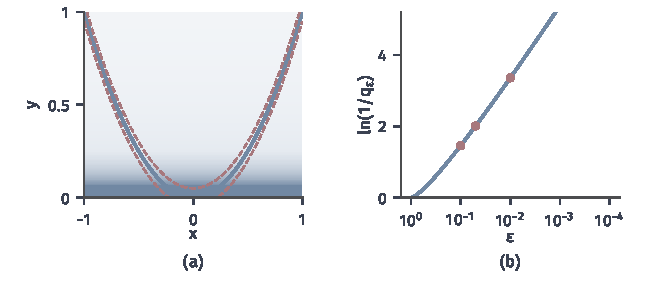
\includegraphics[width=110mm]{figures/07-probability/04-distribution-analysis/matplotlib/dep-graph-band/figure.pdf}
  \caption{质量在曲线上与质量摊开。(a)连续抛物线的边缘乘积密度$1/(4\sqrt{y})$（白到蓝，大于$1$的部分截断显示）；蓝线是联合分布的全部质量所在的曲线$y=x^{2}$，红色虚线围出带子$\lvert y-x^{2}\rvert\leq0.05$。(b)带子在边缘乘积下的概率$q_\varepsilon$给出的下界$\ln(1/q_\varepsilon)$，横轴向右$\varepsilon$减小；红点为$\varepsilon=0.1,0.05,0.01$，对应$1.46$、$2.01$、$3.35$。}
  \label{fig:dep-graph-band}
\end{BookInlineFigure}

下面的定理把“曲线面积为零”换成边缘乘积给图像零概率，给出一般结论。这里要求取值空间是标准Borel空间（第~\ref{chap:conditional-distributions}章引入，欧氏空间及其Borel子集都是），它保证了函数图像可测。

\begin{theorem}[确定关系的互信息]
\label{thm:dep-mi-infinite}
设$\mathcal{X},\mathcal{Y}$是标准Borel空间，$f:\mathcal{X}\to\mathcal{Y}$可测，$Y=f(X)$。若$Y$的分布无原子，即$\mathbb{P}(Y=y)=0$对每个$y\in\mathcal{Y}$成立，则
\begin{equation}
  I\bigl(X;f(X)\bigr)=+\infty .
  \label{eq:dep-mi-infinite}
\end{equation}
\end{theorem}

\begin{proof}
考虑$f$的图像$G=\{(x,y):y=f(x)\}$。标准Borel空间的对角线$\Delta=\{(y,y)\}$是$\mathcal{Y}\times\mathcal{Y}$中的可测集，而$G$是$\Delta$在可测映射$(x,y)\mapsto(f(x),y)$下的原像，所以$G$可测。

联合分布把全部质量放在$G$上：
\[
  P_{(X,Y)}(G)=\mathbb{P}\bigl(f(X)=Y\bigr)=1 .
\]
再算边缘乘积给$G$的概率。由乘积测度的截面公式（Tonelli定理），先固定$x$，截面$\{y:(x,y)\in G\}$只有一个点$f(x)$，于是
\[
  (P_X\otimes P_Y)(G)=\int_{\mathcal{X}}P_Y\bigl(\{f(x)\}\bigr)\,P_X(\mathrm{d}x)=0 ,
\]
最后一步用了$P_Y$无原子。一个集合在$P_X\otimes P_Y$下概率为零、在$P_{(X,Y)}$下概率为一，所以$P_{(X,Y)}$不绝对连续于$P_X\otimes P_Y$，按约定式~\eqref{eq:dep-mi}中的KL散度为$+\infty$。
\end{proof}

定理中两个条件各有作用。无原子保证了边缘乘积给图像零概率；若$Y$有原子，例如三点抛物线，图像的乘积概率为正，互信息有限。标准Borel保证图像可测，从而“质量全在图像上”有意义。函数$f$本身不需要连续或单调：$f(x)=x^{2}$不是一一的，结论照样成立。

\paragraph{有限与无穷的分界}
离散情形的对照是：若$Y=f(X)$只取有限多个值，那么给定$X$后$Y$没有不确定性，
\[
  I\bigl(X;f(X)\bigr)=H\bigl(f(X)\bigr)\leq\ln\lvert f(\mathcal{X})\rvert ,
\]
其中$\lvert f(\mathcal{X})\rvert$是取值个数。三点抛物线$H(Y)=0.637<\ln2$就是这种情形。可数无穷多个取值时，$H(f(X))$可以已经是无穷大；不可数且无原子时，定理~\ref{thm:dep-mi-infinite}说它一定是无穷大。所以互信息没有一个对所有分布都成立的有限上界，它的数值本身不能直接归一化到$[0,1]$。

加一点噪声，互信息又变成有限的。令$Y=X^{2}+\sigma Z$，$Z\sim\mathcal{N}(0,1)$与$X$独立。给定$X=x$时$Y\sim\mathcal{N}(x^{2},\sigma^{2})$，条件微分熵是$\frac12\ln(2\pi\mathrm{e}\sigma^{2})$，所以
\[
  I(X;Y)=h(Y)-\tfrac12\ln(2\pi\mathrm{e}\sigma^{2}),
\]
其中$h(Y)$对$Y$的密度（$X^{2}$的分布与$\mathcal{N}(0,\sigma^{2})$的卷积）数值积分得到。$\sigma=0.2$时约为$0.555$，$\sigma=0.1$时约为$1.03$。$\sigma\to0$时$h(Y)$趋于$X^{2}$的微分熵，而噪声项$-\frac12\ln(2\pi\mathrm{e}\sigma^{2})$像$\ln(1/\sigma)$那样增长，互信息随之发散。高斯情形的$-\frac12\ln(1-\rho^{2})$在$\lvert\rho\rvert\to1$时同样发散。图~\ref{fig:dep-mi-noise}把两种发散画在一起。

\begin{BookInlineFigure}
  \centering
  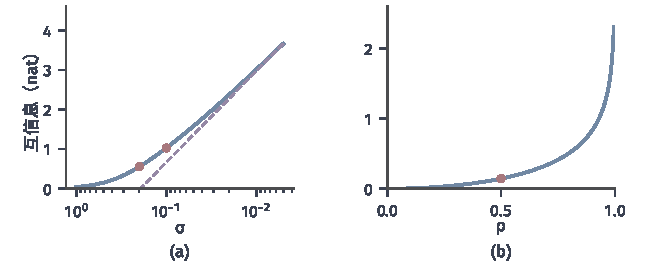
\includegraphics[width=110mm]{figures/07-probability/04-distribution-analysis/matplotlib/dep-mi-noise/figure.pdf}
  \caption{互信息向无穷大发散。(a)$I(X;X^{2}+\sigma Z)$随$\sigma$减小（横轴向右）而增大，蓝线由$h(Y)-\frac12\ln(2\pi\mathrm{e}\sigma^{2})$数值积分得到；紫色虚线是斜率与$\ln(1/\sigma)$相同的参考线；红点为$\sigma=0.2,0.1$，数值约$0.555$、$1.03$。(b)标准二元高斯的$I=-\frac12\ln(1-\rho^{2})$，红点为$\rho=0.5$处的$0.144$。}
  \label{fig:dep-mi-noise}
\end{BookInlineFigure}

\paragraph{下界不是数值}
真实互信息可以无穷大，计算上常用的却是有限的下界。第~\ref{chap:information-measures}章的InfoNCE下界在$N$个候选时不超过$\ln N$：对连续抛物线，$N=16$时它至多给出$\ln16\approx2.77$，而真实值是$+\infty$。下界给出“至少有这么多信息”，不能读成“信息就这么多”；两个分布的下界大小次序，也不一定是它们真实互信息的次序。
